\documentclass[a4 paper]{article}
% Set target color model to RGB
\usepackage[inner=2.0cm,outer=2.0cm,top=2.5cm,bottom=2.5cm]{geometry}
\usepackage{setspace}
\usepackage[rgb]{xcolor}
\usepackage{verbatim}
\usepackage{subcaption}
\usepackage{enumerate}
\usepackage{amsgen,amsmath,amstext,amsbsy,amsopn,tikz,amssymb,tkz-linknodes}
\usepackage{fancyhdr}
\usepackage[colorlinks=true, urlcolor=blue,  linkcolor=blue, citecolor=blue]{hyperref}
\usepackage[colorinlistoftodos]{todonotes}
\usepackage{rotating}
\usepackage{booktabs}

\usepackage{listings}
\lstset{
    language=Python,
    basicstyle=\ttfamily\small,
    aboveskip={1.0\baselineskip},
    belowskip={1.0\baselineskip},
    columns=fixed,
    extendedchars=true,
    breaklines=true,
    tabsize=4,
    prebreak=\raisebox{0ex}[0ex][0ex]{\ensuremath{\hookleftarrow}},
    frame=lines,
    showtabs=false,
    showspaces=false,
    showstringspaces=false,
    keywordstyle=\color[rgb]{0.627,0.126,0.941},
    commentstyle=\color[rgb]{0.133,0.545,0.133},
    stringstyle=\color[rgb]{01,0,0},
    numbers=left,
    numberstyle=\small,
    stepnumber=1,
    numbersep=10pt,
    captionpos=t,
    escapeinside={\%*}{*)}
}

% Command settings
\newcommand{\ra}[1]{\renewcommand{\arraystretch}{#1}}

\newtheorem{thm}{Theorem}[section]
\newtheorem{prop}[thm]{Proposition}
\newtheorem{lem}[thm]{Lemma}
\newtheorem{cor}[thm]{Corollary}
\newtheorem{defn}[thm]{Definition}
\newtheorem{rem}[thm]{Remark}
% \numberwithin{equation}{section}

\newcommand{\homework}[6]{
   \pagestyle{myheadings}
   \thispagestyle{plain}
   \newpage
   \setcounter{page}{1}
   \noindent
   \begin{center}
   \framebox{
      \vbox{\vspace{2mm}
    \hbox to 6.28in { {\bf CS 224n:~Natural Language Processing with Deep Learning \hfill {\small (#3)}} }
       \vspace{6mm}
       \hbox to 6.28in { {\Large \hfill #1 {\small (#2)} \hfill} }
       \vspace{6mm}
       \hbox to 6.28in { {\it Instructor: {\rm #4} \hfill Name: {\rm #5}} }
      \vspace{2mm}}
   }
   \end{center}
   \markboth{\textbf{CS 224n} #1 #2}{\textbf{CS 224n} #1 #2}
   \vspace*{4mm}
}

\newcommand{\problem}[2]{~\\\fbox{\textbf{Problem #1}}\hfill (#2 points)\newline\newline}
\newcommand{\subproblem}[1]{~\newline\textbf{(#1)}}
\newcommand{\solution}{~\newline\textbf{\textit{(Solution)}} }
\newcommand{\bb}[1]{$\boldsymbol{#1}$}
\newcommand{\wtv}{\texttt{word2vec}}


\begin{document}
\homework{Submission Assignment \#2}{word2vec (43 Points)}{Due: 01/21/20}{Christopher Manning}{Jianpan Gun}

\problem{1: Understanding word2vec}{3+5+5+3+4+3=23}

Let's have a quick refresher on the \wtv algorithm.
The key insight behind \wtv is that `a word is known by the company it keeps'.
Concretely, suppose we have a `center' word c and a contextual window surrounding c.
We shall refer to words that lie in this contextual window as `outside words'. 
For example, in Figure 1 we see that the center word c is `banking'.
Since the context window size is 2, the outside words are `turning', `into', `crises', and `as'.

The goal of the skip-gram \wtv algorithm is to accurately learn the probability distribution $P(O|C)$.
Given a specific word o and a specific word c, we want to calculate $P(O = o|C = c)$, which is the probability that word o is an 'outside' word for c, i.e., the probability that o falls within the contextual window of c.

\begin{figure}[h]
    \begin{center}
    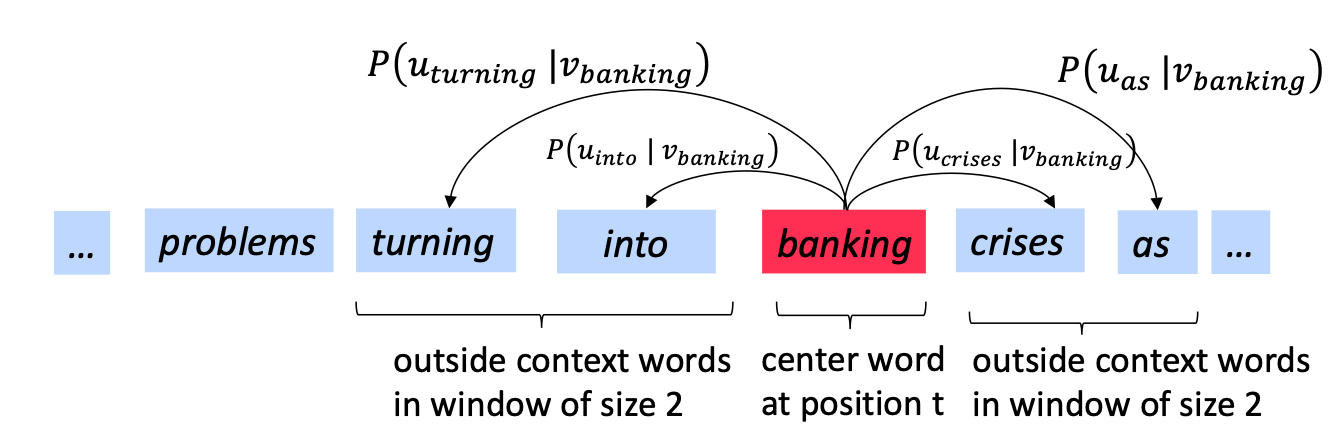
\includegraphics[width=0.8\textwidth]{img/cs224n_assignment.png}
    \caption{The \wtv skip-gram prediction model with window size 2.}
    \label{fig:intro_example}
    \end{center}
\end{figure}

In \wtv, the conditional probability distribution is given by taking vector dot-products and applying the softmax function:

\begin{equation}
    P(O=o | C=c)=\frac{\exp \left(\boldsymbol{u}_{o}^{\top} \boldsymbol{v}_{c}\right)}{\sum_{w \in \mathrm{V_{ocab}}} \exp \left(\boldsymbol{u}_{w}^{\top} \boldsymbol{v}_{c}\right)}
    \label{eq:softmax}
\end{equation}

Here, \bb{u_o} is the `outside' vector representing outside word $o$, and \bb{v_c} is the `center' vector representing center word $c$.
To contain these parameters, we have two matrices, \bb{U} and \bb{V}.
The columns of \bb{U} are all the `outside' vectors \bb{u_w}.
The columns of \bb{V} are all of the `center' vectors \bb{v_w}.
Both \bb{U} and \bb{V} contain a vector for every $w\in$ Vocabulary.

Recall from lectures that, for a single pair of words $c$ and $o$, the loss is given by:
\begin{equation}
    J_{\text {naive-softmax}}\left(\boldsymbol{v}_{c}, o, \boldsymbol{U}\right) = -\log P(O=o | C=c)
    \label{eq:naive-softmax}
\end{equation}

Another way to view this loss is as the cross-entropy between the true distribution \bb{y} and the predicted distribution \bb{\hat{y}}.
Here, both \bb{y} and \bb{\hat{y}} are vectors with length equal to the number of words in the vocabulary.
Furthermore, the $k^{th}$ entry in these vectors indicates the conditional probability of the $k^{th}$ word being an `outside word' for the given $c$.
The true empirical distribution \bb{y} is a one-hot vector with a 1 for the true outside word $o$, and 0 everywhere else.
The predicted distribution \bb{\hat{y}} is the probability distribution $P(O|C = c)$ given by our model in equation (\ref{eq:softmax}).

\subproblem{a} (3 points) \textbf{Show that the naive-softmax loss given in Equation (\ref{eq:naive-softmax}) is the same as the cross-entropy loss between \bb{y} and \bb{\hat{y}}; i.e., show that} $-\sum_{w \in V_{ocab}} y_{w} \log \left(\hat{y}_{w}\right)=-\log \left(\hat{y}_{o}\right)$

\textbf{A}: Due to the \bb{y_i} is a one-hot vector, that is, $\mathbb{I}_{i}$, which means that only have i-th dim is 1.
So,

\begin{equation}
    \mathcal{L}_{ce} = -\sum_{w \in V_{ocab}} y_{w} \log \left(\hat{y}_{w}\right)= -\boldsymbol{y}_o\log \left(\boldsymbol{\hat{y}}_{o}\right) = -\log \left(\hat{y}_{o}\right)
\end{equation}

\subproblem{b} (5 points) \textbf{Compute the partial derivative of $J_{\text {naive-softmax}}\left(\boldsymbol{v}_{c}, o, \boldsymbol{U}\right)$ with respect to \bb{v_c}. Please write your answer in terms of \bb{y}, \bb{\hat{y}}, and \bb{U}}

\begin{equation}
    \begin{aligned}
        \frac{\partial \mathcal J_{\text {naive-softmax}}}{\partial \boldsymbol{v}_c}
        \left(\boldsymbol{v}_{c}, o, \boldsymbol{U}\right)
        = \frac{\partial}{\partial \boldsymbol{v}_c} -\log \frac{\exp \left(\boldsymbol{u}_{o}^{\top} \boldsymbol{v}_{c}\right)}{\sum_{w \in \mathrm{V_{ocab}}} \exp \left(\boldsymbol{u}_{w}^{\top} \boldsymbol{v}_{c}\right)}
        = -\boldsymbol{u}_{o} + \frac{\partial}{\partial \boldsymbol{v}_c} \log \sum_{w \in \mathrm{V_{ocab}}} \exp \left(\boldsymbol{u}_{w}^{\top} \boldsymbol{v}_{c}\right) \\
        = -\boldsymbol{u}_{o} + \frac{1}{\sum_{w \in \mathrm{V_{ocab}}} \exp \left(\boldsymbol{u}_{w}^{\top} \boldsymbol{v}_{c}\right)} \sum_{w \in \mathrm{V_{ocab}}} \exp \left(\boldsymbol{u}_{w}^{\top} \boldsymbol{v}_{c}\right) \boldsymbol{u}_{w} \\
        = -\boldsymbol{y}^\top\boldsymbol{U} + \sum_{w \in \mathrm{V_{ocab}}} P(O=w | C=c) \boldsymbol{u}_{w} \\
        = -\boldsymbol{y}^\top\boldsymbol{U} + \boldsymbol{\hat{y}}^\top\boldsymbol{U}
        = (\boldsymbol{\hat{y}}-\boldsymbol{y})^\top \boldsymbol{U}
    \end{aligned}
\end{equation}

\subproblem{c} (5 points) \textbf{Compute the partial derivatives of $J_{\text {naive-softmax}}\left(\boldsymbol{v}_{c}, o, \boldsymbol{U}\right)$ with respect to each of the `outside' word vectors, \bb{u_w}’s.
There will be two cases: when $w = o$, the true `outside' word vector; and $w\neq o$, for all other words.
Please write you answer in terms of \bb{y}, \bb{\hat{y}}, and \bb{v_c}.}

\begin{equation}
    \begin{aligned}
        \frac{\partial \mathcal J_{\text {naive-softmax}}}{\partial \boldsymbol{u}_w}
        \left(\boldsymbol{v}_{c}, o, \boldsymbol{U}\right)
        = \frac{\partial}{\partial \boldsymbol{u}_w} -\log \frac{\exp \left(\boldsymbol{u}_{o}^{\top} \boldsymbol{v}_{c}\right)}{\sum_{w \in \mathrm{V_{ocab}}} \exp \left(\boldsymbol{u}_{w}^{\top} \boldsymbol{v}_{c}\right)}
        = -\frac{\partial \boldsymbol{u}_{o}^{\top} \boldsymbol{v}_{c}}{\partial \boldsymbol{u}_w} + \frac{\partial}{\partial \boldsymbol{u}_w} \log \sum_{w \in \mathrm{V_{ocab}}} \exp \left(\boldsymbol{u}_{w}^{\top} \boldsymbol{v}_{c}\right)
    \end{aligned}
\end{equation}

If $w=o$:

\begin{equation}
    \begin{aligned}
        = -\boldsymbol{v}_{c} + \frac{\exp \left(\boldsymbol{u}_{o}^{\top} \boldsymbol{v}_{c}\right) \boldsymbol{v}_{c}}{\sum_{w \in \mathrm{V_{ocab}}} \exp \left(\boldsymbol{u}_{w}^{\top} \boldsymbol{v}_{c}\right)}
        = (P(O=o | C=c)- 1)\boldsymbol{v}_{c}
    \end{aligned}
\end{equation}

If $w\neq o$:

\begin{equation}
    \begin{aligned}
        = \frac{\exp \left(\boldsymbol{u}_{w}^{\top} \boldsymbol{v}_{c}\right) \boldsymbol{v}_{c}}{\sum_{w \in \mathrm{V_{ocab}}} \exp \left(\boldsymbol{u}_{w}^{\top} \boldsymbol{v}_{c}\right)}
        = P(O=w | C=c)\boldsymbol{v}_{c}
    \end{aligned}
\end{equation}

So,
\begin{equation}
    \begin{aligned}
        = (\boldsymbol{\hat{y}} - \boldsymbol{y})^\top\boldsymbol{v}_{c}
    \end{aligned}
\end{equation}

\subproblem{d} (3 Points) \textbf{The sigmoid function is given by Equation \ref{eq:sigmoid}:}
\begin{equation}
    \sigma(x)=\frac{1}{1+e^{-x}}=\frac{e^{x}}{e^{x}+1}
    \label{eq:sigmoid}
\end{equation}

\textbf{Please compute the derivative of $\sigma(x)$ with respect to x, where x is a scalar. Hint: you may want to write your answer in terms of $\sigma(x)$.}

\begin{equation}
    \begin{aligned}
        \frac{\partial \sigma(x)}{\partial x}
         = \frac{\partial}{\partial x} \frac{e^{x}}{e^{x}+1}
         = \frac{e^{x} \dot (e^{x}+1) - e^{x} \dot (e^{x}+1)'}{(e^{x}+1)^2}
         = \frac{e^{2x}}{(e^{x}+1)^2}
         = \sigma(x) (1-\sigma(x))
    \end{aligned}
\end{equation}

\subproblem{e} (4 points) \textbf{Now we shall consider the Negative Sampling loss, which is an alternative to the Naive Softmax loss.
Assume that K negative samples (words) are drawn from the vocabulary.
For simplicity of notation we shall refer to them as $w_1,w_2,\dots,w_K$ and their outside vectors as $u_1,\dots,u_K$.
Note that $o\not\in {w_1,\dots,w_K}$.
For a center word c and an outside word $o$, the negative sampling loss function is given by:}
\begin{equation}
    \boldsymbol{J}_{\text {neg-sample}}\left(\boldsymbol{v}_{c}, o, \boldsymbol{U}\right)
    = - \log \left(\sigma\left(\boldsymbol{u}_{o}^{\top} \boldsymbol{v}_{c}\right)\right)-\sum_{k=1}^{K} \log \left(\sigma\left(-\boldsymbol{u}_{k}^{\top} \boldsymbol{v}_{c}\right)\right)
\end{equation}
\textbf{for a sample $w_1,w_2,\dots,w_K$, where $\sigma(\cdot)$ is the sigmoid function.}

\textbf{Please repeat parts (b) and (c), computing the partial derivatives of $\boldsymbol{J}_{\text {neg-sample}}$ with respect to \bb{v_c}, with respect to \bb{u_o}, and with respect to a negative sample \bb{u_k}.
Please write your answers in terms of the vectors \bb{u_o},\bb{v_c}, and \bb{u_k}, where $k \in [1,k]$.
After you've done this, describe with one sentence why this loss function is much more efficient to compute than the naive-softmax loss.
Note, you should be able to use your solution to part (d) to help compute the necessary gradients here.}

\begin{equation}
    \begin{aligned}
        \frac{\partial \mathcal J_{\text {neg-sample}}}{\partial \boldsymbol{v}_c}
        \left(\boldsymbol{v}_{c}, o, \boldsymbol{U}\right)
        = \frac{\partial}{\partial \boldsymbol{v}_c} [- \log \left(\sigma\left(\boldsymbol{u}_{o}^{\top} \boldsymbol{v}_{c}\right)\right) - \sum_{k=1}^{K} \log \left(\sigma\left(-\boldsymbol{u}_{k}^{\top} \boldsymbol{v}_{c}\right)\right)]
        = - \frac{\sigma\left(\boldsymbol{u}_{o}^{\top} \boldsymbol{v}_{c}\right)(1-\sigma\left(\boldsymbol{u}_{o}^{\top} \boldsymbol{v}_{c}\right))\boldsymbol{u}_{o}}{\sigma\left(\boldsymbol{u}_{o}^{\top} \boldsymbol{v}_{c}\right)} \\
        + \sum_{k=1}^{K} \left(1- \sigma\left(-\boldsymbol{u}_{k}^{\top} \boldsymbol{v}_{c}\right)\right)\boldsymbol{u}_{k}
        = -(1-\sigma\left(\boldsymbol{u}_{o}^{\top} \boldsymbol{v}_{c}\right))\boldsymbol{u}_{o} + \sum_{k=1}^{K} \left(1- \sigma\left(-\boldsymbol{u}_{k}^{\top} \boldsymbol{v}_{c}\right)\right)\boldsymbol{u}_{k}
    \end{aligned}
\end{equation}

\begin{equation}
    \begin{aligned}
        \frac{\partial \mathcal J_{\text {neg-sample}}}{\partial \boldsymbol{u}_o}
        \left(\boldsymbol{v}_{c}, o, \boldsymbol{U}\right)
        = \frac{\partial}{\partial \boldsymbol{u}_o} [- \log \left(\sigma\left(\boldsymbol{u}_{o}^{\top} \boldsymbol{v}_{c}\right)\right) - \sum_{k=1}^{K} \log \left(\sigma\left(-\boldsymbol{u}_{k}^{\top} \boldsymbol{v}_{c}\right)\right)]
        = - \frac{\sigma\left(\boldsymbol{u}_{o}^{\top} \boldsymbol{v}_{c}\right)(1-\sigma\left(\boldsymbol{u}_{o}^{\top} \boldsymbol{v}_{c}\right))\boldsymbol{v}_{c}}{\sigma\left(\boldsymbol{u}_{o}^{\top} \boldsymbol{v}_{c}\right)} \\
        = -(1-\sigma\left(\boldsymbol{u}_{o}^{\top} \boldsymbol{v}_{c}\right))\boldsymbol{v}_{c}
    \end{aligned}
\end{equation}

\begin{equation}
    \begin{aligned}
        \frac{\partial \mathcal J_{\text {neg-sample}}}{\partial \boldsymbol{u}_k}
        \left(\boldsymbol{v}_{c}, o, \boldsymbol{U}\right)
        = \frac{\partial}{\partial \boldsymbol{u}_k} [- \log \left(\sigma\left(\boldsymbol{u}_{o}^{\top} \boldsymbol{v}_{c}\right)\right) - \sum_{k=1}^{K} \log \left(\sigma\left(-\boldsymbol{u}_{k}^{\top} \boldsymbol{v}_{c}\right)\right)]
        = \left(1- \sigma\left(-\boldsymbol{u}_{k}^{\top} \boldsymbol{v}_{c}\right)\right)\boldsymbol{v}_{c}
    \end{aligned}
\end{equation}

\subproblem{f} (3 points) \textbf{Suppose the center word is $c = wt$ and the context window is $w_{t-m}, \dots, w_{t-1},w_t,w_{t+1},$ $\dots,w_{t+m}$, where m is the context window size.
Recall that for the skip-gram version of \wtv, the total loss for the context window is:}

\begin{equation}
    J_{\text {skip-gram}}\left(\boldsymbol{v}_{c}, w_{t-m}, \ldots w_{t+m}, \boldsymbol{U}\right)
    =\sum_{-m \leq j \leq m \atop j \neq 0} \boldsymbol{J}\left(\boldsymbol{v}_{c}, w_{t+j}, \boldsymbol{U}\right)
\end{equation}

\textbf{Here, $J\left(\boldsymbol{v}_{c}, w_{t+j}, \boldsymbol{U}\right)$ represents an arbitrary loss term for the center word $c= wt$ and outside word $w_{t+j}$.
$J\left(\boldsymbol{v}_{c}, w_{t+j}, \boldsymbol{U}\right)$ could be $J_{\text{neg-sample}}\left(\boldsymbol{v}_{c}, w_{t+j}, \boldsymbol{U}\right)$ or $J_{\text{naive-softmax}}\left(\boldsymbol{v}_{c}, w_{t+j}, \boldsymbol{U}\right)$, depending on your implementation.}

\textbf{Write down three partial derivatives:}

\begin{enumerate}[(I)]
\item $\partial \boldsymbol{J}_{\text {skip-gram }}\left(\boldsymbol{v}_{c}, w_{t-m}, \ldots w_{t+m}, \boldsymbol{U}\right) / \partial \boldsymbol{U}$
\item $\partial \boldsymbol{J}_{\text {skip-gram }}\left(\boldsymbol{v}_{c}, w_{t-m}, \ldots w_{t+m}, \boldsymbol{U}\right) / \partial \boldsymbol{v}_{c}$
\item $\partial \boldsymbol{J}_{\text {skip-gram }}\left(\boldsymbol{v}_{c}, w_{t-m}, \ldots w_{t+m}, \boldsymbol{U}\right) / \partial \boldsymbol{v}_{w}$, when $w \neq c$
\end{enumerate}

\textbf{Write your answers in terms of $\partial J\left(\boldsymbol{v}_{c}, w_{t+j}, \boldsymbol{U}\right)/\partial U$ and $\partial J\left(\boldsymbol{v}_{c}, w_{t+j}, \boldsymbol{U}\right)/\partial v_c$.
This is very simple.
Each solution should be one line.
Once you’re done: Given that you computed the derivatives of $J\left(\boldsymbol{v}_{c}, w_{t+j}, \boldsymbol{U}\right)$ with respect to all the model parameters \bb{U} and \bb{V} in parts (a) to (c), you have now computed the derivatives of the full loss function $J_{skip-gram}$ with respect to all parameters.
You’re ready to implement \wtv!}

(I) 

For native-softmax:
\begin{equation}
    \begin{aligned}
        \frac{\partial J_{\text {skip-gram}} }{\partial \boldsymbol{U}}
        \left(\boldsymbol{v}_{c}, o, \boldsymbol{U}\right)
        = \sum_{-m \leq j \leq m \atop j \neq 0} (\boldsymbol{\hat{y}} - \boldsymbol{y})^\top\boldsymbol{v}_{j}
    \end{aligned}
\end{equation}

For neg-sample:
\begin{equation}
    \begin{aligned}
        \frac{\partial J_{\text {skip-gram}} }{\partial \boldsymbol{U}}
        \left(\boldsymbol{v}_{c}, o, \boldsymbol{U}\right)
        = \sum_{-m \leq j \leq m \atop j \neq 0} (1-\sigma\left(\boldsymbol{u}_{o}^{\top} \boldsymbol{v}_{j}\right))\boldsymbol{v}_{j}
    \end{aligned}
\end{equation}

(II) 

For native-softmax:
\begin{equation}
    \begin{aligned}
        \frac{\partial J_{\text {skip-gram}} }{\partial \boldsymbol{v}_c}
        \left(\boldsymbol{v}_{c}, o, \boldsymbol{U}\right)
        = \sum_{-m \leq j \leq m \atop j \neq 0} (\boldsymbol{\hat{y}}-\boldsymbol{y})^\top \boldsymbol{U}
    \end{aligned}
\end{equation}

For neg-sample:
\begin{equation}
    \begin{aligned}
        \frac{\partial J_{\text {skip-gram}} }{\partial \boldsymbol{v}_c}
        \left(\boldsymbol{v}_{c}, o, \boldsymbol{U}\right)
        = \sum_{-m \leq j \leq m \atop j \neq 0} (-(1-\sigma\left(\boldsymbol{u}_{o}^{\top} \boldsymbol{v}_{j}\right))\boldsymbol{u}_{o} + \sum_{k=1}^{K} \left(1- \sigma\left(-\boldsymbol{u}_{k}^{\top} \boldsymbol{v}_{j}\right)\right)\boldsymbol{u}_{k})
    \end{aligned}
\end{equation}

(III) 

\begin{equation}
    \begin{aligned}
        \frac{\partial J_{\text {skip-gram}} }{\partial \boldsymbol{v}_w}
        \left(\boldsymbol{v}_{c}, o, \boldsymbol{U}\right)
        = 0
    \end{aligned}
\end{equation}

\problem{Implementing word2vec (20 points)}{12+4+4=20}

\subproblem{a} (12 points) \textbf{We will start by implementing methods in \texttt{word2vec.py}.
First, implement the \texttt{sigmoid} method, which takes in a vector and applies the sigmoid function to it.
Then implement the softmax loss and gradient in the \texttt{naiveSoftmaxLossAndGradient} method, and negative sampling loss and gradient in the \texttt{negSamplingLossAndGradient} method.
Finally, fill in the implementation for the skip-gram model in the \texttt{skipgram} method.
When you are done, test your implementation by running python \texttt{word2vec.py}}

\begin{lstlisting}[label={list:first},caption=word2vec.py function.]
def sigmoid(x):
    # \sigma(x)=\frac{1}{1+e^{-x}}=\frac{e^{x}}{e^{x}+1}
    s = 1 / (1 + np.exp(-x))
    return s
    
def naiveSoftmaxLossAndGradient(centerWordVec, outsideWordIdx, outsideVectors, dataset):
    y_hat = softmax(np.dot(centerWordVec, outsideVectors.T)) 

    loss = -np.log(y_hat[outsideWordIdx]) # ref to equation(2)
    y = np.zeros_like(y_hat)
    y[outsideWordIdx] = 1
    gradCenterVec = np.dot((y_hat - y).T, outsideVectors) # ref to equation(4)
    gradOutsideVecs = np.dot(
        (y_hat - y).reshape(-1, 1), centerWordVec.reshape(1, -1)
    )  # (T, 1) * (1, H) ref to equation(8)

    return loss, gradCenterVec, gradOutsideVecs
    
def negSamplingLossAndGradient(
    centerWordVec, outsideWordIdx, outsideVectors, dataset, K=10
):
    negSampleWordIndices = getNegativeSamples(outsideWordIdx, dataset, K)
    indices = [outsideWordIdx] + negSampleWordIndices

    negSampleWordIndices = np.array(negSampleWordIndices)

    pos = sigmoid(np.dot(outsideVectors[outsideWordIdx], centerWordVec))
    neg = sigmoid(-np.dot(outsideVectors[negSampleWordIndices], centerWordVec))
    loss = -np.log(pos) - np.log(neg).sum() # ref to equation(11)
    gradCenterVec = -np.dot((1 - pos), outsideVectors[outsideWordIdx]) + np.dot(
        1 - neg, outsideVectors[negSampleWordIndices]
    ) # ref to equation(12)
    gradOutsideVecs = np.zeros_like(outsideVectors)
    gradOutsideVecs[outsideWordIdx] = - np.dot(1 - pos, centerWordVec) # ref to equation(13)
    gradOutside = np.dot((1 - neg).reshape(-1, 1), centerWordVec.reshape(1, -1))
    for idx, neg_idx in enumerate(negSampleWordIndices):
        gradOutsideVecs[neg_idx] += gradOutside[idx] # ref to equation(14)

    return loss, gradCenterVec, gradOutsideVecs

def skipgram(
    currentCenterWord,
    windowSize,
    outsideWords,
    word2Ind,
    centerWordVectors,
    outsideVectors,
    dataset,
    word2vecLossAndGradient=naiveSoftmaxLossAndGradient,
):
    loss = 0.0
    gradCenterVecs = np.zeros(centerWordVectors.shape)
    gradOutsideVectors = np.zeros(outsideVectors.shape)

    centerWordIdx = word2Ind[currentCenterWord]
    centerWordVector = centerWordVectors[centerWordIdx]
    for outsideWord in outsideWords:
        outsideWordIdx = word2Ind[outsideWord]
        tmp_loss, gradCenterVec, gradOutsideVector = word2vecLossAndGradient(
            centerWordVector, outsideWordIdx, outsideVectors, dataset
        )
        loss += tmp_loss
        gradCenterVecs[centerWordIdx, :] += gradCenterVec # ref to equation(18,19)
        gradOutsideVectors += gradOutsideVector

    return loss, gradCenterVecs, gradOutsideVectors
\end{lstlisting}

\subproblem{b} (4 points) \textbf{Complete the implementation for your \texttt{SGD} optimizer in the \texttt{sgd} method of \texttt{sgd.py}.
Test your implementation by running python \texttt{sgd.py}.}

\begin{lstlisting}[label={list:first},caption=sgd.py function.]

def sgd(f, x0, step, iterations, postprocessing=None, useSaved=False, PRINT_EVERY=10):
    # Anneal learning rate every several iterations
    ANNEAL_EVERY = 20000

    if useSaved:
        start_iter, oldx, state = load_saved_params()
        if start_iter > 0:
            x0 = oldx
            step *= 0.5 ** (start_iter / ANNEAL_EVERY)

        if state:
            random.setstate(state)
    else:
        start_iter = 0

    x = x0

    if not postprocessing:
        postprocessing = lambda x: x

    exploss = None

    for iter in range(start_iter + 1, iterations + 1):
        # You might want to print the progress every few iterations.

        # c, gin, gout = word2vecModel(
        #     centerWord,
        #     windowSize1,
        #     context,
        #     word2Ind,
        #     centerWordVectors,
        #     outsideVectors,
        #     dataset,
        #     word2vecLossAndGradient,
        # )
        # loss += c / batchsize
        # grad[: int(N / 2), :] += gin / batchsize
        # grad[int(N / 2) :, :] += gout / batchsi
        loss, grad = f(x)
        x -= step * grad

        x = postprocessing(x)
        if iter % PRINT_EVERY == 0:
            if not exploss:
                exploss = loss
            else:
                exploss = 0.95 * exploss + 0.05 * loss
            print("iter %d: %f" % (iter, exploss))

        if iter % SAVE_PARAMS_EVERY == 0 and useSaved:
            save_params(iter, x)

        if iter % ANNEAL_EVERY == 0:
            step *= 0.5
    return x
\end{lstlisting}

\subproblem{c} (4 points) \textbf{Show time! Now we are going to load some real data and train word vectors with everything you just implemented!
We are going to use the \texttt{Stanford Sentiment Treebank (SST)} dataset to train word
vectors, and later apply them to a simple sentiment analysis task.
You will need to fetch the datasets first.
To do this, run sh get \texttt{datasets.sh}.
There is no additional code to write for this part; just run python \texttt{run.py}.}

\begin{figure}[h]
    \begin{center}
    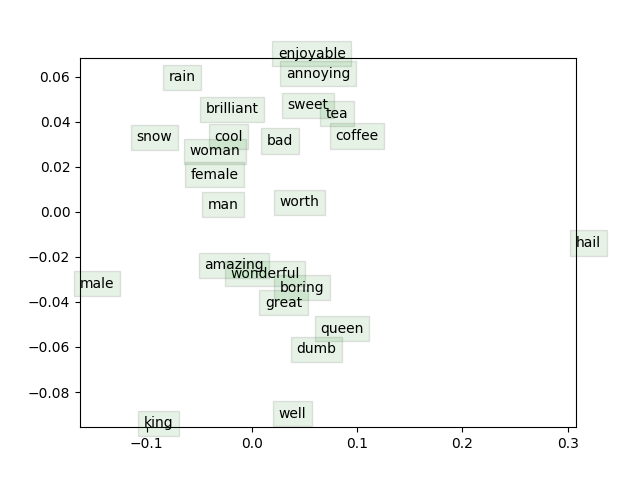
\includegraphics[width=0.6\textwidth]{img/word_vectors.png}
    \caption{The word vector distribution figure.}
    \label{fig:intro_example}
    \end{center}
\end{figure}

\end{document} 
